\documentclass[a4paper,twoside,10pt,landscape]{article}
\usepackage{multicol}
\usepackage{calc}
\usepackage{ifthen}
\usepackage[landscape]{geometry}
\usepackage{hyperref}
\usepackage{graphicx} % standard LaTeX graphics tool when including figure files
\graphicspath{{images/}}
\usepackage[font={small}]{caption}
\captionsetup{aboveskip=3pt}

% To make this come out properly in landscape mode, do one of the following
% 1.
%  pdflatex latexsheet.tex
%
% 2.
%  latex latexsheet.tex
%  dvips -P pdf  -t landscape latexsheet.dvi
%  ps2pdf latexsheet.ps


% If you're reading this, be prepared for confusion.  Making this was
% a learning experience for me, and it shows.  Much of the placement
% was hacked in; if you make it better, let me know...


% 2008-04
% Changed page margin code to use the geometry package. Also added code for
% conditional page margins, depending on paper size. Thanks to Uwe Ziegenhagen
% for the suggestions.

% 2006-08
% Made changes based on suggestions from Gene Cooperman. <gene at ccs.neu.edu>


% To Do:
% \listoffigures \listoftables
% \setcounter{secnumdepth}{0}


% This sets page margins to .5 inch if using letter paper, and to 1cm
% if using A4 paper. (This probably isn't strictly necessary.)
% If using another size paper, use default 1cm margins.
\ifthenelse{\lengthtest { \paperwidth = 11in}}
	{ \geometry{top=.5in,left=.5in,right=.5in,bottom=.5in} }
	{\ifthenelse{ \lengthtest{ \paperwidth = 297mm}}
		{\geometry{top=1cm,left=1cm,right=1cm,bottom=1cm} }
		{\geometry{top=1cm,left=1cm,right=1cm,bottom=1cm} }
	}

% Turn off header and footer
\pagestyle{empty}
 

% Redefine section commands to use less space
\makeatletter
\renewcommand{\section}{\@startsection{section}{1}{0mm}%
                                {-1ex plus -.5ex minus -.2ex}%
                                {0.5ex plus .2ex}%x
                                {\normalfont\large\bfseries}}
\renewcommand{\subsection}{\@startsection{subsection}{2}{0mm}%
                                {-1explus -.5ex minus -.2ex}%
                                {0.5ex plus .2ex}%
                                {\normalfont\normalsize\bfseries}}
\renewcommand{\subsubsection}{\@startsection{subsubsection}{3}{0mm}%
                                {-1ex plus -.5ex minus -.2ex}%
                                {1ex plus .2ex}%
                                {\normalfont\small\bfseries}}
\makeatother

% Define BibTeX command
\def\BibTeX{{\rm B\kern-.05em{\sc i\kern-.025em b}\kern-.08em
    T\kern-.1667em\lower.7ex\hbox{E}\kern-.125emX}}

% Don't print section numbers
%\setcounter{secnumdepth}{0}


\setlength{\parindent}{0pt}
\setlength{\parskip}{0pt plus 0.5ex}


% -----------------------------------------------------------------------

\begin{document}

\raggedright
\footnotesize
\begin{multicols}{3}


% multicol parameters
% These lengths are set only within the two main columns
%\setlength{\columnseprule}{0.25pt}
\setlength{\premulticols}{1pt}
\setlength{\postmulticols}{1pt}
\setlength{\multicolsep}{1pt}
\setlength{\columnsep}{2pt}

\begin{center}
     \Large{\textbf{Scala Cheat Sheet}} \\
\end{center}


\section{Scala Class Hierarchy}
\begin{center}
    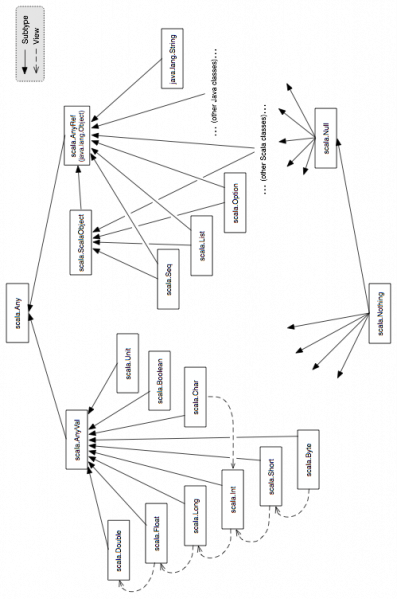
\includegraphics[scale=.69]{classhierarchy.png}
    \captionof{figure}{Scala class hierarchy, source: \url{http://www.scala-lang.org/old/node/128}}
    \label{fig:scala-class-hierarchy}
\end{center}


\section{Scala Collections}


\subsection{Scala Collections Hierarchy}

\begin{center}
    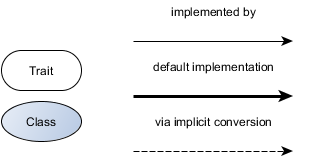
\includegraphics[scale=.50]{legend.png}
\end{center}

\begin{center}
    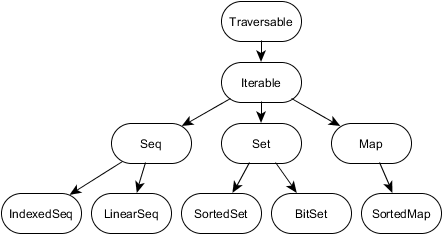
\includegraphics[scale=.50]{scala-collection.png}
    \captionof{figure}{scala.collection}
    \label{fig:scala-collection}
\end{center}

\begin{center}
    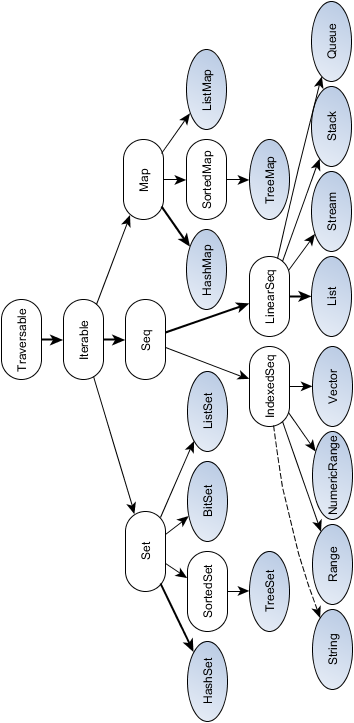
\includegraphics[scale=.70]{scala-collection-immutable.png}
    \captionof{figure}{scala.collection.immutable}
    \label{fig:scala-collection-immutable}
\end{center}

\begin{center}
    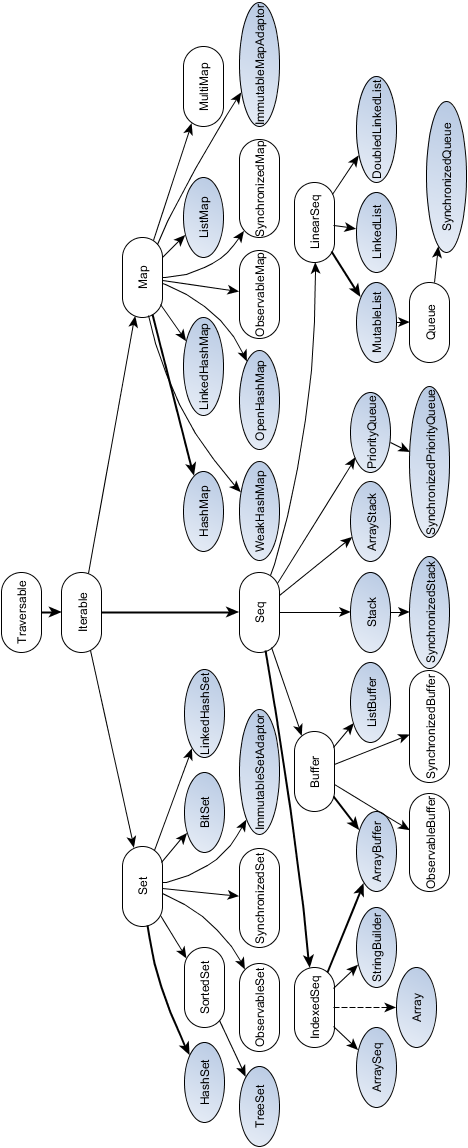
\includegraphics[scale=.68]{scala-collection-mutable.png}
    \captionof{figure}{scala.collection.mutable}
    \label{fig:scala-collection-mutable}
\end{center}


\subsection{Trait \texttt{Traversable}}
\begin{center}
\captionof{table}{Methods in \texttt{Traversable}}
\begin{tabular}{@{}lp{6.5cm}@{}}
\hline\noalign{\smallskip}
\textbf{Category} & \textbf{Methods} \\
\noalign{\smallskip}\hline\noalign{\smallskip}
\textbf{Abstract} & \texttt{xs foreach f}\\
\textbf{Addition} & \texttt{xs ++ ys}\\
\textbf{Maps} & \texttt{xs map f, xs flatMap f, xs collect f}\\
\textbf{Conversions} & \texttt{toArray, toList, toIterable, toSeq, toIndexedSeq, toStream, toSet, toMap}\\
\textbf{Size info} & \texttt{isEmpty, nonEmpty, size, hasDefiniteSize}\\
\textbf{Element} & \texttt{head, headOption, last, lastOption},\\
\textbf{Retrieval} & \texttt{xs find p}\\
\textbf{Sub-} & \texttt{xs.tail, xs.init, xs slice (from, to)},\\
\textbf{collection} & \texttt{xs take n, xs drop n, xs takeWhile p, xs dropWhile p, xs filter p, xs withFilter p, xs filterNot p}\\
\textbf{Subdivision} & \texttt{xs splitAt n, xs span p, xs partition p, xs groupBy f}\\
\textbf{Element} & \texttt{xs forall p, xs exists p, xs count p}\\
\textbf{Condition} & \\
\textbf{Fold} & \texttt{(z /: xs)(op), (xs :\ z)(op), xs.foldLeft(z)(op), xs.foldRight(z)(op), xs reduceLeft op, xs reduceRight op}\\
\textbf{Specific Fold} & \texttt{xs.sum, xs.product, xs.min, xs.max}\\
\textbf{String} & \texttt{xs addString (b, start, sep, end), xs mkString (start, sep, end), xs.stringPrefix}\\
\textbf{View} & \texttt{xs.view, xs view (from, to)}\\
\noalign{\smallskip}\hline
\end{tabular}
\raggedright{\tiny{Reference: \url{http://docs.scala-lang.org/overviews/collections/trait-traversable.html}}}
\end{center}


\subsection{Trait \texttt{Iterable}}
All methods in this trait are defined in terms of an an abstract method, \texttt{iterator}, which yields the collection’s elements one by one.

\begin{center}
\captionof{table}{Methods in \texttt{Iterable}}
\begin{tabular}{@{}lp{6cm}@{}}
\hline\noalign{\smallskip}
\textbf{Category} & \textbf{Methods} \\
\noalign{\smallskip}\hline\noalign{\smallskip}
\textbf{Abstract} & \texttt{xs.iterator}\\
\textbf{Iterator} & \texttt{xs grouped n, xs sliding n}\\
\textbf{Subcollection} & \texttt{xs takeRight n, xs dropRight n}\\
\textbf{Zipper} & \texttt{xs zip ys, xs zipAll (ys, x, y), xs.zipWithIndex}\\
\textbf{Comparison} & \texttt{xs sameElements ys}\\
\noalign{\smallskip}\hline
\end{tabular}
\raggedright{\tiny{Reference: \url{http://docs.scala-lang.org/overviews/collections/trait-iterable.html}}}
\end{center}

In the inheritance hierarchy below \texttt{Iterable} you find three traits: \texttt{Seq}, \texttt{Set}, and \texttt{Map}. A common aspect of these three traits is that they all implement the \texttt{PartialFunction} trait with its \texttt{apply} and \texttt{isDefinedAt} methods. However, the way each trait implements \texttt{PartialFunction} differs.


\subsection{Seq}

\begin{center}
\captionof{table}{Methods in \texttt{Seq}}
\begin{tabular}{@{}lp{6.5cm}@{}}
\hline\noalign{\smallskip}
\textbf{Category} & \textbf{Methods} \\
\noalign{\smallskip}\hline\noalign{\smallskip}
\textbf{Indexing and} & \texttt{xs(i), xs isDefinedAt i, xs.length,}\\
\textbf{Length} & \texttt{xs.lengthCompare ys, xs.indices}\\
\textbf{Index Search} & \texttt{xs indexOf x, xs lastIndexOf x, xs indexOfSlice ys, xs lastIndexOfSlice ys, xs indexWhere p, xs segmentLength (p, i), xs prefixLength p}\\
\textbf{Addition} & \texttt{x +: xs, xs :+ x, xs padTo (len, x)}\\
\textbf{Update} & \texttt{xs patch (i, ys, r), xs updated (i, x), xs(i) = x}(only available for \texttt{mutable.Seq}s)\\
\textbf{Sorting} & \texttt{xs.sorted, xs sortWith lt, xs sortBy f}\\
\textbf{Reversal} & \texttt{xs.reverse, xs.reverseIterator, xs reverseMap f}\\
\textbf{Comparison} & \texttt{xs startsWith ys, xs endsWith ys, xs contains x, xs containsSlice ys, (xs corresponds ys)(p)}\\
\textbf{Multiset} & \texttt{xs intersect ys, xs union ys, xs diff ys, xs.distinct}\\
\noalign{\smallskip}\hline
\end{tabular}
\raggedright{\tiny{Reference: \url{http://docs.scala-lang.org/overviews/collections/seqs.html}}}
\end{center}

\begin{center}
\captionof{table}{Methods in \texttt{Buffer}}
\begin{tabular}{@{}lp{6.5cm}@{}}
\hline\noalign{\smallskip}
\textbf{Category} & \textbf{Methods} \\
\noalign{\smallskip}\hline\noalign{\smallskip}
\textbf{Addition} & \texttt{buf += x, buf += (x, y, z), buf ++= xs, x +=: buf, xs ++=: buf, buf insert (i, x), buf insertAll (i, xs)}\\
\textbf{Removal} & \texttt{buf -= x, buf remove i, buf remove (i, n), buf trimStart n, buf trimEnd n, buf.clear()}\\
\textbf{Cloning} & \texttt{buf.clone}\\
\noalign{\smallskip}\hline
\end{tabular}
\end{center}


\subsection{Set}
\begin{center}
\captionof{table}{Methods in \texttt{Set}}
\begin{tabular}{@{}lp{6.5cm}@{}}
\hline\noalign{\smallskip}
\textbf{Category} & \textbf{Methods} \\
\noalign{\smallskip}\hline\noalign{\smallskip}
\textbf{Test} & \texttt{xs contains x, xs(x), xs subsetOf ys}\\
\textbf{Addition} & \texttt{xs + x, xs + (x, y, z), xs ++ ys}\\
\textbf{Removal} & \texttt{xs - x, xs - (x, y, z), xs -- ys, xs.empty}\\
\textbf{Set operation} & \texttt{xs \& ys, xs intersect ys, xs | ys, xs union ys, xs \&~ ys, xs diff ys}\\
\noalign{\smallskip}\hline
\end{tabular}
\raggedright{\tiny{Reference: \url{http://docs.scala-lang.org/overviews/collections/sets.html}}}
\end{center}

Mutable sets offer in addition methods to add, remove, or update elements, which are summarized in below.

\begin{center}
\captionof{table}{Methods in \texttt{mutable.Set}}
\begin{tabular}{@{}lp{6.5cm}@{}}
\hline\noalign{\smallskip}
\textbf{Category} & \textbf{Methods} \\
\noalign{\smallskip}\hline\noalign{\smallskip}
\textbf{Addition} & \texttt{xs += x, xs += (x, y, z), xs ++= ys, xs add x}\\
\textbf{Removal} & \texttt{xs -= x, xs -= (x, y, z), xs --= ys, xs remove x, xs retain p, xs.clear()}\\
\textbf{Update} & \texttt{xs(x) = b}\\
\textbf{Cloning} & \texttt{xs.clone}\\
\noalign{\smallskip}\hline
\end{tabular}
\end{center}


\subsection{Map}
\begin{center}
\captionof{table}{Methods in \texttt{Map}}
\begin{tabular}{@{}lp{6cm}@{}}
\hline\noalign{\smallskip}
\textbf{Category} & \textbf{Methods} \\
\noalign{\smallskip}\hline\noalign{\smallskip}
\textbf{Lookup} & \texttt{ms get k, ms(k), ms getOrElse (k, d), ms contains k, ms isDefinedAt k}\\
\textbf{Addition} & \texttt{ms + (k -> v), ms + (k -> v, l -> w), ms ++ kvs}\\
\textbf{Removal} & \texttt{ms - k, ms - (k, 1, m), ms -- ks}\\
\textbf{Update} & \texttt{ms updated (k, v)}\\
\textbf{Subcollection} & \texttt{ms.keys, ms.keySet, ms.keyIterator, ms.values, ms.valuesIterator}\\
\textbf{Transformation} & \texttt{ms filterKeys p, ms mapValues f}\\
\noalign{\smallskip}\hline
\end{tabular}
\raggedright{\tiny{Reference: \url{http://docs.scala-lang.org/overviews/collections/maps.html}}}
\end{center}

\begin{center}
\captionof{table}{Methods in \texttt{mutable.Map}}
\begin{tabular}{@{}lp{6cm}@{}}
\hline\noalign{\smallskip}
\textbf{Category} & \textbf{Methods} \\
\noalign{\smallskip}\hline\noalign{\smallskip}
\textbf{Addition} & \texttt{ms += (k -> v), ms += (k -> v, l -> w), ms ++= kvs, }\\
\textbf{Removal} & \texttt{ms -= k, ms -= (k, l, m), ms --= ks, ms remove k, ms retain p, ms.clear()}\\
\textbf{Update} & \texttt{ms(k) = v, ms put (k, v), ms getOrElseUpdate (k, d)}\\
\textbf{Transformation} & \texttt{ms transform f}\\
\textbf{Cloning} & \texttt{xs.clone}\\
\noalign{\smallskip}\hline
\end{tabular}
\end{center}


\subsection{Performance Characteristics}
\begingroup
\setlength{\tabcolsep}{1pt}
\begin{center}
\captionof{table}{Performance characteristics of sequence types}
%\begin{tabular}{@{}l@{\hskip 2pt}c@{\hskip 2pt}c@{\hskip 2pt}c@{\hskip 2pt}c@{\hskip 2pt}c@{\hskip 2pt}c@{\hskip 2pt}c@{}}
\begin{tabular}{@{}lccccccc@{}}
\hline\noalign{\smallskip}
 & \textbf{head} & \textbf{tail} & \textbf{apply} & \textbf{update} & \textbf{prepend} & \textbf{append} & \textbf{insert}\\
\noalign{\smallskip}\hline\noalign{\smallskip}
\textbf{immutable} &&&&&&& \\	
\texttt{List} & C & C & L & L & C & L & - \\
\texttt{Stream} & C & C & L & L & C & L & - \\
\texttt{Vector} & eC & eC & eC & eC & eC & eC & - \\
\texttt{Stack} & C & C & L & L & C & C & L \\
\texttt{Queue} & aC & aC & L & L & L & C & - \\
\texttt{Range} & C & C & C & - & - & - & - \\
\texttt{String} & C & L & C & L & L & L & - \\
\textbf{mutable} &&&&&&& \\				
\texttt{ArrayBuffer} & C & L & C & C & L & aC & L \\
\texttt{ListBuffer} & C & L & L & L & C & C & L \\
\texttt{StringBuilder} & C & L & C & C & L & aC & L \\
\texttt{MutableList} & C & L & L & L & C & C & L \\
\texttt{Queue} & C & L & L & L & C & C & L \\
\texttt{ArraySeq} & C & L & C & C & - & - & - \\
\texttt{Stack} & C & L & L & L & C & L & L \\
\texttt{ArrayStack} & C & L & C & C & aC & L & L \\
\texttt{Array} & C & L & C & C & - & - & - \\
\noalign{\smallskip}\hline
\end{tabular}
\raggedright{\tiny{Reference: \url{http://docs.scala-lang.org/overviews/collections/performance-characteristics.html}}}
\end{center}
\endgroup

\begin{center}
\captionof{table}{Performance characteristics of set and map types}
\begin{tabular}{@{}lcccc@{}}
\hline\noalign{\smallskip}
 & \textbf{lookup} & \textbf{add} & \textbf{remove} & \textbf{min} \\
\noalign{\smallskip}\hline\noalign{\smallskip}
\textbf{immutable} &&&& \\
\texttt{HashSet/HashMap} & eC & eC & eC & L \\
\texttt{TreeSet/TreeMap} & Log & Log & Log & Log \\
\texttt{BitSet} & C & L & L & $eC^1$ \\
\texttt{ListMap} & L & L & L & L \\
\textbf{mutable} &&&& \\
\texttt{HashSet/HashMap} & eC & eC & eC & L \\
\texttt{WeakHashMap} & eC & eC & eC & L \\
\texttt{BitSet} & C & aC & C & $eC^1$ \\
\texttt{TreeSet} & Log & Log & Log & Log \\
\noalign{\smallskip}\hline
\multicolumn{5}{c}{\small{Footnote 1: Assuming bits are densely packed.}}
\end{tabular}
\end{center}

The entries in these two tables are explained as follows:

\begin{tabular}{@{}lp{7cm}@{}}
C & The operation takes (fast) constant time. \\
eC & The operation takes effectively constant time, but this might depend on some assumptions such as maximum length of a vector or distribution of hash keys. \\
aC & The operation takes amortized constant time. Some invocations of the operation might take longer, but if many operations are performed on average only constant time per operation is taken. \\
Log & The operation takes time proportional to the logarithm of the collection size. \\
L & The operation is linear, that is it takes time proportional to the collection size. \\
- & The operation is not supported.
\end{tabular}


\section{Scala Parallel Collections}


\subsection{Creating a Parallel Collection}
Two ways to create a parallel collection: \texttt{new} and \texttt{par}.


\subsection{Semantics}
Conceptually, Scala’s parallel collections framework parallelizes an operation on a parallel collection by recursively “splitting” a given collection, applying an operation on each partition of the collection in parallel, and re-“combining” all of the results that were completed in parallel.

These concurrent, and “out-of-order” semantics of parallel collections lead to the following two implications:
\begin{enumerate}
\item Side-effecting operations can lead to non-determinism
\item Non-associative operations lead to non-determinism
\end{enumerate}


\subsection{Concrete Parallel Collection Classes}
\texttt{mutable.ParArray}, \texttt{immutable.ParVector}, \texttt{immutable.ParRange}, 

\texttt{mutable.ParHashSet}, \texttt{mutable.ParHashMap}, \texttt{immutable.ParHashSet}, \texttt{immutable.ParHashMap}, 

\texttt{mutable.ParTrieMap}


\subsection{Performance characteristics}
\begingroup
\setlength{\tabcolsep}{1pt}
\begin{center}
\captionof{table}{Performance characteristics of sequence types}
\begin{tabular}{@{}lccccccc@{}}
\hline\noalign{\smallskip}
 & \textbf{head} & \textbf{tail} & \textbf{apply} & \textbf{update} & \textbf{prepend} & \textbf{append} & \textbf{insert}\\
\noalign{\smallskip}\hline\noalign{\smallskip}
\texttt{ParArray} & C & L & C & C & L & L & L \\
\texttt{ParVector} & eC & eC & eC & eC & eC & eC & - \\
\texttt{ParRange} & C & C & C & - & - & - & - \\
\noalign{\smallskip}\hline
\end{tabular}
\raggedright{\tiny{\url{http://docs.scala-lang.org/overviews/parallel-collections/concrete-parallel-collections.html}}}
\end{center}
\endgroup

\begin{center}
\captionof{table}{Performance characteristics of set and map types}
\begin{tabular}{@{}lcccc@{}}
\hline\noalign{\smallskip}
 & \textbf{lookup} & \textbf{add} & \textbf{remove} \\
\noalign{\smallskip}\hline\noalign{\smallskip}
\textbf{immutable} &&& \\
\texttt{ParHashSet/ParHashMap} & eC & eC & eC \\
\textbf{mutable} &&& \\
\texttt{ParHashSet/ParHashMap} & C & C & C \\
\texttt{ParTrieMap} & eC & eC & eC \\
\noalign{\smallskip}\hline
\end{tabular}
\end{center}


\subsection{Parallel Collection Conversions}
Every sequential collection can be converted to its parallel variant using the \texttt{par} method. Certain sequential collections have a direct parallel counterpart. For these collections the conversion is efficient– it occurs in constant time, since both the sequential and the parallel collection have the same data-structural representation (one exception is mutable hash maps and hash sets which are slightly more expensive to convert the first time \texttt{par} is called, but subsequent invocations of par take constant time). It should be noted that for mutable collections, changes in the sequential collection are visible in its parallel counterpart if they share the underlying data-structure.

\begin{center}
\captionof{table}{Sequential collections and their direct parallel counterparts}
\begin{tabular}{@{}ll@{}}
\hline\noalign{\smallskip}
\textbf{Sequential} & \textbf{Parallel} \\
\noalign{\smallskip}\hline\noalign{\smallskip}
\textbf{mutable} & \\
\texttt{Array} & \texttt{ParArray} \\
\texttt{HashMap} & \texttt{ParHashMap} \\
\texttt{HashSet} & \texttt{ParHashSet} \\
\texttt{TrieMap} & \texttt{ParTrieMap} \\
\textbf{immutable} & \\
\texttt{Vector} & \texttt{ParVector} \\
\texttt{Range} & \texttt{ParRange} \\
\texttt{HashMap} & \texttt{ParHashMap} \\
\texttt{HashSet} & \texttt{ParHashSet} \\
\noalign{\smallskip}\hline
\end{tabular} \\
\raggedright{\tiny{Source: \url{http://docs.scala-lang.org/overviews/parallel-collections/conversions.html}}}
\end{center}

Other collections, such as lists, queues or streams, are inherently sequential in the sense that the elements must be accessed one after the other. These collections are converted to their parallel variants by copying the elements into a similar parallel collection. For example, a functional list is converted into a standard immutable parallel sequence, which is a parallel vector.

Every parallel collection can be converted to its sequential variant using the \texttt{seq} method. Converting a parallel collection to a sequential collection is always efficient– it takes constant time. Calling seq on a mutable parallel collection yields a sequential collection which is backed by the same store– updates to one collection will be visible in the other one.


\subsection{Architecture of the Parallel Collections Library}
Two core abstractions: \texttt{Splitter}s and \texttt{Combiner}s.

\textbf{Splitter}
\begin{verbatim}
trait Splitter[T] extends Iterator[T] {
  def split: Seq[Splitter[T]]
}
\end{verbatim}

\textbf{Combiner}
\begin{verbatim}
trait Combiner[Elem, To] extends Builder[Elem, To] {
  def combine(other: Combiner[Elem, To]): Combiner[Elem, To]
}
\end{verbatim}



\rule{0.3\linewidth}{0.25pt}
\scriptsize

Copyright \copyright\ 2014 soulmachine

Github: \url{https://github.com/soulmachine/scala-cheat-sheet} 

My blog: \url{http://www.soulmachine.me}

Last update: \today


\end{multicols}
\end{document}
